% ===============================================================================
% SEQUENCE OVERVIEW - 10 Double Lessons Leading to Observation Feb 2026
% Spanish Late-Starters (Kl. 10, 11, 12) - Cross-Grade Course
% ===============================================================================

\documentclass[11pt, a4paper]{article}

\usepackage[utf8]{inputenc}
\usepackage[T1]{fontenc}
\usepackage[english]{babel}
\usepackage{helvet}
\renewcommand{\familydefault}{\sfdefault}

\usepackage[margin=1.5cm, top=1.5cm, bottom=1.5cm]{geometry}
\usepackage[table]{xcolor}
\usepackage{array}
\usepackage{tabularx}
\usepackage{longtable}
\usepackage{booktabs}
\usepackage{tikz}
\usepackage{amssymb}
\usepackage{enumitem}
\usepackage{fancyhdr}
\usepackage{lastpage}

% Colors
\definecolor{spanisch}{HTML}{c41e3a}
\definecolor{grau}{HTML}{666666}
\definecolor{hellgrau}{HTML}{f5f5f5}
\definecolor{gruppeA}{HTML}{2a7a4b}
\definecolor{gruppeB}{HTML}{1565c0}
\definecolor{puffer}{HTML}{6a0dad}
\definecolor{assessment}{HTML}{b35c00}
\definecolor{beobachtung}{HTML}{c41e3a}
\definecolor{success}{HTML}{2a7a4b}

% Spanish command
\newcommand{\es}[1]{\textcolor{spanisch}{\textit{#1}}}

% Header and footer
\pagestyle{fancy}
\fancyhf{}
\renewcommand{\headrulewidth}{0.4pt}
\lhead{\small Sequence Overview -- Spanish Late-Starters}
\rhead{\small Observation February 2026}
\cfoot{\small Page \thepage\ of \pageref{LastPage}}

\setlength{\parindent}{0pt}

\begin{document}

% ===============================================================================
% TITLE PAGE
% ===============================================================================

\begin{center}
{\color{spanisch}\rule{\textwidth}{2pt}}\\[0.8cm]
{\Huge\bfseries SEQUENCE OVERVIEW}\\[0.3cm]
{\Large Spanish Late-Starters -- 10 Double Lessons}\\[0.5cm]
{\large Preparation for External Observation}\\[0.2cm]
{\large\bfseries February 3, 2026}\\[0.5cm]
{\color{spanisch}\rule{\textwidth}{2pt}}
\end{center}

\vspace{0.5cm}

% ===============================================================================
% COURSE INFORMATION
% ===============================================================================

\begin{center}
\begin{tabular}{|p{4cm}|p{11cm}|}
\hline
\rowcolor{hellgrau}
\textbf{Course} & Spanish Late-Starters (cross-grade) \\
\hline
\textbf{Grade Levels} & 10, 11, 12 \\
\hline
\textbf{Class Size} & 10 students (1 male, 9 female) \\
\hline
\textbf{Textbook} & A\_tope.com (Cornelsen) \\
\hline
\textbf{Weekly Hours} & 4 (Mon + Tue, double lessons each) \\
\hline
\rowcolor{hellgrau}
\textbf{Differentiation} & \textcolor{gruppeA}{\textbf{Group A}} (7 students): Year 1, A2 level \quad \textcolor{gruppeB}{\textbf{Group B}} (3 students): Year 2--3, B1 level \\
\hline
\end{tabular}
\end{center}

\vspace{0.5cm}

% ===============================================================================
% TIMELINE
% ===============================================================================

\begin{center}
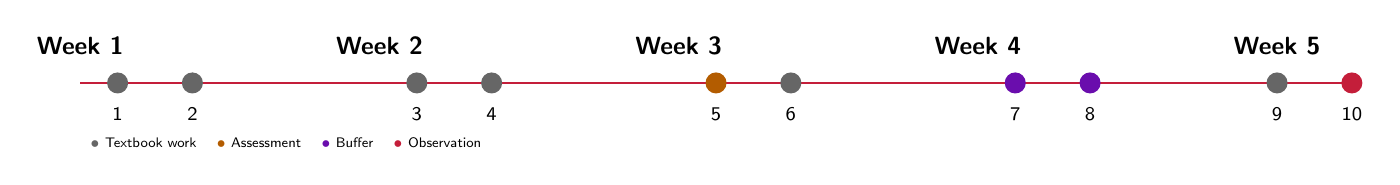
\begin{tikzpicture}[scale=0.95]
% Week headers
\node[font=\small\bfseries] at (0,0.5) {Week 1};
\node[font=\small\bfseries] at (4,0.5) {Week 2};
\node[font=\small\bfseries] at (8,0.5) {Week 3};
\node[font=\small\bfseries] at (12,0.5) {Week 4};
\node[font=\small\bfseries] at (16,0.5) {Week 5};

% Timeline
\draw[thick, spanisch] (0,0) -- (17,0);

% Points and labels
\fill[grau] (0.5,0) circle (4pt); \node[font=\scriptsize, below] at (0.5,-0.2) {1};
\fill[grau] (1.5,0) circle (4pt); \node[font=\scriptsize, below] at (1.5,-0.2) {2};
\fill[grau] (4.5,0) circle (4pt); \node[font=\scriptsize, below] at (4.5,-0.2) {3};
\fill[grau] (5.5,0) circle (4pt); \node[font=\scriptsize, below] at (5.5,-0.2) {4};
\fill[assessment] (8.5,0) circle (4pt); \node[font=\scriptsize, below] at (8.5,-0.2) {5};
\fill[grau] (9.5,0) circle (4pt); \node[font=\scriptsize, below] at (9.5,-0.2) {6};
\fill[puffer] (12.5,0) circle (4pt); \node[font=\scriptsize, below] at (12.5,-0.2) {7};
\fill[puffer] (13.5,0) circle (4pt); \node[font=\scriptsize, below] at (13.5,-0.2) {8};
\fill[grau] (16,0) circle (4pt); \node[font=\scriptsize, below] at (16,-0.2) {9};
\fill[beobachtung] (17,0) circle (4pt); \node[font=\scriptsize, below] at (17,-0.2) {10};

% Legend
\node[font=\tiny, right] at (0,-0.8) {
    \textcolor{grau}{$\bullet$} Textbook work \quad
    \textcolor{assessment}{$\bullet$} Assessment \quad
    \textcolor{puffer}{$\bullet$} Buffer \quad
    \textcolor{beobachtung}{$\bullet$} Observation
};
\end{tikzpicture}
\end{center}

\vspace{0.5cm}

% ===============================================================================
% COMPACT OVERVIEW TABLE
% ===============================================================================

{\large\bfseries\color{spanisch} Overview of All 10 Double Lessons}

\vspace{0.3cm}

\renewcommand{\arraystretch}{1.4}
\small
\begin{longtable}{|c|p{2.2cm}|p{3.5cm}|p{4cm}|p{4cm}|}
\hline
\rowcolor{spanisch}
\textcolor{white}{\textbf{DL}} &
\textcolor{white}{\textbf{Date}} &
\textcolor{white}{\textbf{Topic}} &
\textcolor{white}{\textbf{Learning Objectives}} &
\textcolor{white}{\textbf{Special Notes}} \\
\hline
\endfirsthead
\hline
\rowcolor{spanisch}
\textcolor{white}{\textbf{DL}} &
\textcolor{white}{\textbf{Date}} &
\textcolor{white}{\textbf{Topic}} &
\textcolor{white}{\textbf{Learning Objectives}} &
\textcolor{white}{\textbf{Special Notes}} \\
\hline
\endhead

\textbf{1} & Jan 05 (Mon) & Parallel textbook work &
A: Vocabulary \es{Mi barrio}, \es{hay} + location; B: Profession vocabulary, \es{ser/estar} &
First lesson after break, reactivation \\
\hline

\textbf{2} & Jan 06 (Tue) & Continuation + Transition &
Consolidate lesson content, listening comprehension, shared vocabulary &
First shared element, B students as experts \\
\hline

\textbf{3} & Jan 12 (Mon) & Textbook work + Announcement &
Complete lessons, understand assessment criteria &
\textcolor{assessment}{Assessment info!} Criteria discussion \\
\hline

\textbf{4} & Jan 13 (Tue) & Final textbook work &
A: Secure \es{hay/ser/estar}; B: Structure short presentation &
\textcolor{assessment}{Last practice before assessment!} \\
\hline

\rowcolor{yellow!20}
\textbf{5} & Jan 19 (Mon) & \textbf{ASSESSMENT} &
A: Dialog \es{Mi barrio}; B: Short presentation \es{Mi profesion ideal} &
\textcolor{assessment}{\textbf{Graded assessment!}} 25 pts $\rightarrow$ 15 NP \\
\hline

\textbf{6} & Jan 20 (Tue) & Bridge topic &
\es{ser} vs. \es{estar} + adjective, describing people &
\textcolor{gruppeB}{B students as tutors!} Mixed tandems \\
\hline

\rowcolor{purple!10}
\textbf{7} & Jan 26 (Mon) & \textcolor{puffer}{Culture \& Fun} &
Cultural knowledge, apply vocabulary, motivation &
\textcolor{puffer}{\textbf{BUFFER!}} No new content. Online available \\
\hline

\rowcolor{purple!10}
\textbf{8} & Jan 27 (Tue) & \textcolor{puffer}{Creativity \& Games} &
Creative person descriptions, writing skills &
\textcolor{puffer}{\textbf{BUFFER!}} \es{Mi persona favorita}. Online available \\
\hline

\textbf{9} & Feb 02 (Mon) & Review \& Preparation &
Review \es{ser/estar/hay}, know procedure, build confidence &
Day before observation! Practice run \\
\hline

\rowcolor{red!15}
\textbf{10} & Feb 03 (Tue) & \textbf{OBSERVATION} &
Communicative competence, correct \es{ser/estar}, 3rd person &
\textcolor{beobachtung}{\textbf{EXTERNAL OBSERVATION!}} Tandem interview \\
\hline

\end{longtable}

\normalsize
\renewcommand{\arraystretch}{1.0}

\vspace{0.3cm}

% ===============================================================================
% DETAILED DESCRIPTIONS
% ===============================================================================

{\large\bfseries\color{spanisch} Detailed Lesson Descriptions}

\vspace{0.3cm}

% PHASE 1
\textbf{\color{spanisch} PHASE 1: Textbook Work \& Assessment (DL 1--5)}

\vspace{0.2cm}

% ---------------------------------------------------------------------------
% DL 1
% ---------------------------------------------------------------------------
\fbox{\parbox{0.97\textwidth}{
\textbf{DL 1 -- Parallel Textbook Work} (January 5, 2026)\\[0.2cm]

\textbf{Learning Objectives:}
\begin{itemize}[nosep, leftmargin=1.5em]
    \item Group A: Learn neighborhood vocabulary, use \es{hay} + location, formulate questions with \es{vuestro}
    \item Group B: Review profession vocabulary, apply \es{ser/estar} in context
\end{itemize}

\textbf{Lesson Flow:}
\begin{tabular}{p{1.5cm}p{12cm}}
0--5 min & Welcome, daily overview, confirm group setup \\
5--20 min & A: Exercise 9 (vuestro questions); B: Exercise 6a (school system) \\
20--35 min & Teacher rotates: A continues dialog prep; B explains Spanish system \\
35--50 min & A: Partner dialog Madrid (p. 136); B: German system comparison \\
50--65 min & A: Dialog presentation; B: Mediation exercise \\
65--80 min & A: Blog entry (\es{Mi barrio}); B: Complete mediation task \\
80--90 min & Summary, homework assignment \\
\end{tabular}

\textbf{Activities:} Textbook work, partner dialog exercises, written exercises, self-check

\textbf{Pedagogical Intention:} Differentiated instruction allows both groups to progress at appropriate levels while the teacher rotates attention.

\textbf{Special Notes:} First lesson after winter break. Reactivation focus. Teacher rotates between groups every 10--15 minutes. E.H. can serve as peer tutor in Group A.
}}

\vspace{0.3cm}

% ---------------------------------------------------------------------------
% DL 2
% ---------------------------------------------------------------------------
\fbox{\parbox{0.97\textwidth}{
\textbf{DL 2 -- Continuation + Transition} (January 6, 2026)\\[0.2cm]

\textbf{Learning Objectives:}
\begin{itemize}[nosep, leftmargin=1.5em]
    \item Consolidate lesson content from DL 1
    \item Practice listening comprehension
    \item Introduce first shared vocabulary element between groups
\end{itemize}

\textbf{Lesson Flow:}
\begin{tabular}{p{1.5cm}p{12cm}}
0--10 min & Warm-up: Vocabulary review game (all together) \\
10--30 min & A: Listening exercise from textbook; B: Complete comparison task \\
30--50 min & Shared element: Kahoot/Quizlet vocabulary game (mixed groups) \\
50--70 min & Introduction: \es{ser} + adjective (describing people) \\
70--85 min & Practice in mixed pairs: B students help A students \\
85--90 min & Reflection, homework \\
\end{tabular}

\textbf{Activities:} Textbook work, listening exercise, shared vocabulary game (Kahoot/Quizlet), introduction to \es{ser} + adjective

\textbf{Pedagogical Intention:} Create first bridge between the two groups through a shared activity. B students begin to take on expert/helper roles for A students.

\textbf{Special Notes:} First shared element. B students as experts for A students. This prepares the collaborative dynamic needed for the observation lesson.
}}

\vspace{0.3cm}

% ---------------------------------------------------------------------------
% DL 3
% ---------------------------------------------------------------------------
\fbox{\parbox{0.97\textwidth}{
\textbf{DL 3 -- Textbook Work + Assessment Announcement} (January 12, 2026)\\[0.2cm]

\textbf{Learning Objectives:}
\begin{itemize}[nosep, leftmargin=1.5em]
    \item Complete respective textbook lessons
    \item Understand assessment criteria and format
    \item Know what is expected for the assessment (DL 5)
\end{itemize}

\textbf{Lesson Flow:}
\begin{tabular}{p{1.5cm}p{12cm}}
0--5 min & Warm-up, agenda for today \\
5--25 min & Continue/complete textbook lessons (A: p. 32--33; B: p. 104--105) \\
25--40 min & \textcolor{assessment}{\textbf{Assessment Announcement:}} Explain format, distribute criteria sheets \\
40--60 min & Practice assessment format: A practices dialog; B practices presentation \\
60--80 min & Peer feedback on practice attempts \\
80--90 min & Questions, clarification, homework \\
\end{tabular}

\textbf{Activities:} Textbook work, assessment announcement, criteria discussion, practice formats

\textbf{Pedagogical Intention:} Transparency about expectations reduces anxiety and allows students to prepare appropriately. Clear criteria enable self-assessment.

\textbf{Special Notes:} \textcolor{assessment}{Assessment info!} Students receive criteria sheet. Format: A = partner exam (dialog), B = short presentation.
}}

\vspace{0.3cm}

% ---------------------------------------------------------------------------
% DL 4
% ---------------------------------------------------------------------------
\fbox{\parbox{0.97\textwidth}{
\textbf{DL 4 -- Final Textbook Work Before Assessment} (January 13, 2026)\\[0.2cm]

\textbf{Learning Objectives:}
\begin{itemize}[nosep, leftmargin=1.5em]
    \item Group A: Secure use of \es{hay/ser/estar}
    \item Group B: Structure a short presentation effectively
    \item All: Practice assessment format with peer feedback
\end{itemize}

\textbf{Lesson Flow:}
\begin{tabular}{p{1.5cm}p{12cm}}
0--5 min & Warm-up, focus on assessment preparation \\
5--30 min & A: Grammar review \es{hay/ser/estar}; B: Presentation structure practice \\
30--50 min & A: Partner dialogs (multiple rounds with different partners) \\
50--70 min & B: Practice presentations (2--3 minutes each) \\
70--85 min & Peer feedback, self-assessment \\
85--90 min & Final tips, encouragement \\
\end{tabular}

\textbf{Activities:} A: Partner dialogs practice; B: Presentation rehearsal; mutual peer feedback; self-assessment

\textbf{Pedagogical Intention:} Intensive practice session ensures all students feel prepared. Multiple practice rounds build confidence and automaticity.

\textbf{Special Notes:} \textcolor{assessment}{Last practice before assessment!} Teacher provides individual feedback. Focus on encouragement and constructive tips.
}}

\vspace{0.3cm}

% ---------------------------------------------------------------------------
% DL 5 - ASSESSMENT
% ---------------------------------------------------------------------------
\fcolorbox{assessment}{yellow!10}{\parbox{0.95\textwidth}{
\textbf{\color{assessment} DL 5 -- ASSESSMENT (Graded Performance)} (January 19, 2026)\\[0.2cm]

\textbf{Learning Objectives:}
\begin{itemize}[nosep, leftmargin=1.5em]
    \item Group A: Conduct a partner dialog about \es{Mi barrio}
    \item Group B: Deliver a short presentation about \es{Mi profesion ideal}
    \item Demonstrate communicative competence at respective levels
\end{itemize}

\textbf{Assessment Details:}
\begin{itemize}[nosep, leftmargin=1.5em]
    \item \textbf{Duration:} 45 minutes assessment + 45 minutes productive waiting time
    \item \textbf{Total Points:} 25 BE (Bewertungseinheiten)
    \item \textbf{Grading Scale:} 15-point scale (Abitur system)
\end{itemize}

\textbf{Lesson Flow:}
\begin{tabular}{p{1.5cm}p{12cm}}
0--5 min & Welcome, seating arrangement, final instructions \\
5--10 min & \textcolor{gruppeB}{Group B}: First presentation (3 min + 2 min Q\&A) \\
10--15 min & Group B: Second presentation \\
15--20 min & Group B: Third presentation \\
20--25 min & Transition, \textcolor{gruppeA}{Group A} pairs prepare \\
25--32 min & A Pair 1: Partner dialog (5 min) \\
32--39 min & A Pair 2: Partner dialog \\
39--46 min & A Pair 3: Partner dialog \\
46--53 min & A Pair 4: Partner dialog \\
53--60 min & Buffer time for delays \\
60--90 min & Productive waiting: Self-study, vocabulary review, or quiet reading \\
\end{tabular}

\textbf{Format:}
\begin{itemize}[nosep, leftmargin=1.5em]
    \item \textcolor{gruppeA}{Group A:} Partner exam \es{Mi barrio} (5 min dialog, 2 students)
    \item \textcolor{gruppeB}{Group B:} Short presentation \es{Mi profesion ideal} (3 min presentation + 2 min questions)
\end{itemize}

\textbf{Assessment Criteria:} Content (30\%), Vocabulary (25\%), Grammar (20\%), Fluency/Presentation (25\%)

\textbf{Pedagogical Intention:} Differentiated assessment allows each group to demonstrate competence at their level. Partner format for A reduces anxiety; presentation format for B challenges their higher proficiency.

\textbf{Special Notes:} Grading sheets prepared. Timer visible. Clear rotation system. Students not being assessed work silently on provided materials.
}}

\vspace{0.4cm}

% PHASE 2
\textbf{\color{spanisch} PHASE 2: Convergence \& Buffer (DL 6--8)}

\vspace{0.2cm}

% ---------------------------------------------------------------------------
% DL 6
% ---------------------------------------------------------------------------
\fbox{\parbox{0.97\textwidth}{
\textbf{DL 6 -- Bridge Topic: People and Characteristics} (January 20, 2026)\\[0.2cm]

\textbf{Learning Objectives:}
\begin{itemize}[nosep, leftmargin=1.5em]
    \item Understand and apply \es{ser} vs. \es{estar} with adjectives
    \item Describe people using physical and character adjectives
    \item Practice question-answer format: \es{?Como eres?}
\end{itemize}

\textbf{Lesson Flow:}
\begin{tabular}{p{1.5cm}p{12cm}}
0--10 min & Warm-up: Assessment debrief, positive feedback \\
10--25 min & Shared input: \es{ser} vs. \es{estar} with adjectives (examples on board) \\
25--40 min & Adjective collection: Physical + character traits (collaborative brainstorm) \\
40--55 min & Partner work \es{?Como eres?} -- mixed tandems (A + B) \\
55--75 min & Game: \es{?Quien es?} (guess the person based on descriptions) \\
75--90 min & Reflection, preview of buffer week \\
\end{tabular}

\textbf{Activities:} Shared input on ser vs. estar, adjective collection, partner work \es{?Como eres?}, guessing game \es{?Quien es?}

\textbf{Pedagogical Intention:} First fully shared topic brings both groups together. B students support A students as tutors, building collaborative dynamics for the observation lesson.

\textbf{Special Notes:} \textcolor{gruppeB}{B students as tutors!} Mixed tandems for peer support. This lesson directly prepares for the observation lesson format.
}}

\vspace{0.3cm}

% ---------------------------------------------------------------------------
% DL 7 - BUFFER
% ---------------------------------------------------------------------------
\fcolorbox{puffer}{purple!5}{\parbox{0.95\textwidth}{
\textbf{\color{puffer} DL 7 -- BUFFER: Culture \& Fun} (January 26, 2026)\\[0.2cm]

\textbf{Learning Objectives:}
\begin{itemize}[nosep, leftmargin=1.5em]
    \item Expand cultural knowledge about Spanish-speaking countries
    \item Apply learned vocabulary in playful contexts
    \item Maintain motivation through varied, low-pressure activities
\end{itemize}

\textbf{Lesson Flow:}
\begin{tabular}{p{1.5cm}p{12cm}}
0--10 min & Warm-up: Quick vocabulary review \\
10--30 min & Cultural quiz: Spanish-speaking countries, traditions, geography \\
30--50 min & Spanish music: Listen, identify vocabulary, discuss themes \\
50--70 min & Vocabulary Bingo (review all learned vocabulary) \\
70--85 min & Short film clip with comprehension tasks \\
85--90 min & Reflection on cultural insights \\
\end{tabular}

\textbf{Activities:} Cultural quiz, Spanish music listening, vocabulary Bingo, short film with tasks

\textbf{Pedagogical Intention:} Buffer lesson provides flexibility in the sequence. No new exam-relevant content reduces pressure while maintaining engagement and vocabulary activation.

\textbf{Special Notes:} \textcolor{puffer}{BUFFER WEEK!} No new content. If cancelled: \texttt{ONLINE-07-cultura.html} available for self-study.
}}

\vspace{0.3cm}

% ---------------------------------------------------------------------------
% DL 8 - BUFFER
% ---------------------------------------------------------------------------
\fcolorbox{puffer}{purple!5}{\parbox{0.95\textwidth}{
\textbf{\color{puffer} DL 8 -- BUFFER: Creativity \& Games} (January 27, 2026)\\[0.2cm]

\textbf{Learning Objectives:}
\begin{itemize}[nosep, leftmargin=1.5em]
    \item Apply person descriptions creatively
    \item Practice writing skills at differentiated levels
    \item Share work with peers in a supportive environment
\end{itemize}

\textbf{Lesson Flow:}
\begin{tabular}{p{1.5cm}p{12cm}}
0--10 min & Warm-up: Quick round of person descriptions \\
10--35 min & Writing task: \es{Mi persona favorita} (A: 60--80 words; B: 100--120 words) \\
35--55 min & Peer review in pairs \\
55--75 min & Voluntary presentations + Padlet sharing \\
75--85 min & Games: Vocabulary relay, charades with adjectives \\
85--90 min & Preview of preparation lesson \\
\end{tabular}

\textbf{Activities:} Creative writing (A: 60--80 words, B: 100--120 words), voluntary presentation, Padlet, games

\textbf{Pedagogical Intention:} Creative application reinforces vocabulary without test pressure. Differentiated word counts accommodate different proficiency levels.

\textbf{Special Notes:} \textcolor{puffer}{BUFFER WEEK!} No new structures. If cancelled: \texttt{ONLINE-08-creatividad.html} available for self-study.
}}

\vspace{0.4cm}

% PHASE 3
\textbf{\color{spanisch} PHASE 3: Preparation \& Observation (DL 9--10)}

\vspace{0.2cm}

% ---------------------------------------------------------------------------
% DL 9
% ---------------------------------------------------------------------------
\fbox{\parbox{0.97\textwidth}{
\textbf{DL 9 -- Vocabulary \& Grammar Games} (February 2, 2026)\\[0.2cm]

\fcolorbox{spanisch}{hellgrau}{\parbox{0.93\textwidth}{
\centering
\textbf{IMPORTANT:} Completely different approach from DL 10!\\
No tandem interviews, no ``dress rehearsal'' -- Students should not repeat the same activity.
}}

\vspace{0.2cm}

\textbf{Learning Objectives:}
\begin{itemize}[nosep, leftmargin=1.5em]
    \item Review \es{ser/estar/hay} through games
    \item Master vocabulary (adjectives, professions, hobbies)
    \item Build confidence through varied activities
\end{itemize}

\textbf{Lesson Flow:}
\begin{tabular}{p{1.5cm}p{12cm}}
0--10 min & Warm-up: Adjective chain (``I am... and...'') \\
10--30 min & \textbf{Vocabulary Bingo:} Adjectives + Professions (fun, no pressure!) \\
30--45 min & \textbf{Grammar Stations:} ser vs. estar exercises (3 stations) \\
45--50 min & \textit{Break} \\
50--70 min & \textbf{Writing Exercise:} Short text about favorite star (3rd person) \\
70--80 min & Read texts aloud, peer feedback \\
80--85 min & \textbf{Brief Announcement:} Verbally explain tomorrow's format (5 min only) \\
85--90 min & Positive send-off, answer questions \\
\end{tabular}

\textbf{Activities:} Vocabulary Bingo, grammar stations, writing exercise (3rd person practice), brief verbal announcement

\textbf{Pedagogical Intention:} Practice 3rd person through writing (preparation without rehearsal). Games reduce stress. Tomorrow's format is only mentioned verbally -- NO demonstration!

\textbf{Special Notes:} Day before observation! Different activities than DL 10 so the observation lesson feels fresh, not rehearsed. Students practice the skills without repeating the format.
}}

\vspace{0.3cm}

% ---------------------------------------------------------------------------
% DL 10 - OBSERVATION
% ---------------------------------------------------------------------------
\fcolorbox{beobachtung}{red!5}{\parbox{0.95\textwidth}{
\textbf{\color{beobachtung} DL 10 -- OBSERVATION LESSON} (February 3, 2026)\\[0.2cm]

\textbf{Learning Objectives:}
\begin{itemize}[nosep, leftmargin=1.5em]
    \item Demonstrate communicative competence in Spanish
    \item Use \es{ser/estar} correctly to describe people
    \item Present a partner in 3rd person (\es{el/ella es...})
\end{itemize}

\textbf{Observation Details:}
\begin{itemize}[nosep, leftmargin=1.5em]
    \item \textbf{Observer:} External examiner (for teacher certification)
    \item \textbf{Observed portion:} Second half (45 minutes)
    \item \textbf{Format:} Tandem interviews with mixed A+B pairs, followed by presentations
\end{itemize}

\textbf{Lesson Flow (Full 90 Minutes):}

\textit{First Half (not observed):}
\begin{tabular}{p{1.5cm}p{12cm}}
0--5 min & Welcome, remind of procedure \\
5--20 min & \textbf{Phase 1: Homogeneous tandems} -- A with A, B with B (warm-up) \\
20--40 min & Continue Phase 1, build confidence \\
40--45 min & Transition to mixed tandems, observer arrives \\
\end{tabular}

\textit{Second Half (observed -- 45 minutes):}
\begin{tabular}{p{1.5cm}p{12cm}}
0--3 min & Brief orientation, explain phases, show timer \\
3--15 min & \textbf{Phase 1: Homogeneous pairs} (A with A, B with B) -- 12 min \\
15--33 min & \textbf{Phase 2: Mixed tandems} -- B interviews A using \textbf{checkbox template} -- 18 min \\
33--42 min & \textbf{Phase 3: Presentations} -- \textbf{Only 3 pre-selected tandems} present -- 9 min \\
42--45 min & \textbf{Cierre} -- Summary, farewell in Spanish \\
\end{tabular}

\vspace{0.2cm}

\fcolorbox{success}{success!10}{\parbox{0.93\textwidth}{
\textbf{Timing Optimization:} Checkbox template instead of free writing = faster. Only 3 pre-selected tandems present = no time overrun.
}}

\textbf{Differentiated Question Cards:}
\begin{itemize}[nosep, leftmargin=1.5em]
    \item Group A cards: 3 questions (simpler structures)
    \item Group B cards: 4 questions (more complex)
    \item \textbf{Checkbox summary template} for quick note-taking (no slow writing!)
\end{itemize}

\textbf{Alternative Lesson Plans (Backup):}
\begin{itemize}[nosep, leftmargin=1.5em]
    \item \textbf{Variant A (Standard):} Tandem Interview + Checkbox template -- Score 9.4/10
    \item \textbf{Variant B:} Speed-Dating (6 rounds x 3 min, no writing) -- Low risk, Score 8.7/10
    \item \textbf{Variant C:} Gallery Walk (Poster + presentations) -- Low risk, Score 9.0/10
\end{itemize}

\textbf{Pedagogical Intention:} The mixed tandem format showcases differentiation in action. B students support A students while all demonstrate meaningful communication. The 3rd person presentation adds linguistic challenge.

\textbf{Special Notes:} \textcolor{beobachtung}{EXTERNAL OBSERVATION!} Question cards differentiated (A: 3 / B: 4 questions). B students as tutors. Poster \es{ser vs. estar} visible on board. Seating pre-planned. Alternative plans B and C available as backup.
}}

\newpage

% ===============================================================================
% GRAMMAR PROGRESSION
% ===============================================================================

{\large\bfseries\color{spanisch} Grammar Progression}

\vspace{0.3cm}

\begin{center}
\begin{tabular}{|p{3cm}|p{5.5cm}|p{5.5cm}|}
\hline
\rowcolor{hellgrau}
\textbf{Structure} & \textbf{Group A (A2)} & \textbf{Group B (B1)} \\
\hline
\es{ser} + adjective & DL 2: Introduction (describing people) & DL 1: Review (already known) \\
\hline
\es{estar} + adjective & DL 6: Introduction (states) & DL 1: Review (already known) \\
\hline
\es{hay} + location & DL 1: Introduction (\es{Mi barrio}) & -- (already known) \\
\hline
\es{gustar} & DL 2: Review & DL 1: Application (hobbies) \\
\hline
\es{querer ser} & -- & DL 1--4: Focus (career aspirations) \\
\hline
3rd person singular & DL 6: Introduction (\es{el/ella es...}) & DL 6: Application (presentation) \\
\hline
\end{tabular}
\end{center}

\vspace{0.5cm}

% ===============================================================================
% MATERIALS
% ===============================================================================

{\large\bfseries\color{spanisch} Available Materials}

\vspace{0.3cm}

\begin{tabular}{@{}p{4cm}p{5cm}p{6cm}@{}}
\textbf{Type} & \textbf{Files} & \textbf{Description} \\
\hline
Lesson Plans & LE-01 to LE-10 (.tex/.pdf) & Approx. 8--10 pages each, Tier 1 (complete) \\
Online Tasks & ONLINE-07, -08, -09 (.html) & For buffer week / absences \\
Question Cards & MATERIAL-10-fragekarten.pdf & 6x A, 6x B, summary template, poster \\
Assessment Sheets & MATERIAL-05-bewertungsboegen.pdf & Assessment rubrics, grading scale \\
Materials Overview & UEBERSICHT-materialien.pdf & Complete materials list with checklist \\
This Overview & SEQUENCE-overview.pdf & Compact lesson sequence overview \\
German Version & SEQUENZ-uebersicht.pdf & German version of this document \\
\end{tabular}

\vspace{0.5cm}

% ===============================================================================
% CHECKLIST
% ===============================================================================

{\large\bfseries\color{spanisch} Pre-Observation Checklist}

\vspace{0.3cm}

\begin{tabular}{|p{0.5cm}|p{14cm}|}
\hline
$\Box$ & All 10 lesson plans printed and ready \\
\hline
$\Box$ & Question cards A and B laminated (6 each) \\
\hline
$\Box$ & Poster \es{ser vs. estar} on the board \\
\hline
$\Box$ & Tandem assignment list ready for teacher \\
\hline
$\Box$ & Timer/clock visible \\
\hline
$\Box$ & Assessment sheets for DL 5 printed \\
\hline
$\Box$ & Online tasks tested (ONLINE-07, -08, -09) \\
\hline
$\Box$ & Seating arrangement for mixed tandems planned \\
\hline
$\Box$ & DL 9 completed (vocabulary/grammar games, NO practice run) \\
\hline
$\Box$ & Observer informed about class composition and differentiation approach \\
\hline
\end{tabular}

\vspace{0.5cm}

% ===============================================================================
% KEY PEDAGOGICAL PRINCIPLES
% ===============================================================================

{\large\bfseries\color{spanisch} Key Pedagogical Principles}

\vspace{0.3cm}

\begin{enumerate}[leftmargin=2em]
    \item \textbf{Differentiation by Design:} Two proficiency groups work on level-appropriate content while progressing toward shared communicative goals.

    \item \textbf{Peer Tutoring:} B students (more advanced) systematically support A students, reinforcing their own learning while helping others.

    \item \textbf{Gradual Convergence:} The sequence moves from parallel work (DL 1--5) through bridge activities (DL 6) to fully integrated work (DL 10).

    \item \textbf{Transparent Assessment:} Criteria are shared in advance (DL 3), practice opportunities are provided (DL 4), and formats match proficiency levels.

    \item \textbf{Buffer Flexibility:} DL 7--8 provide flexibility for unexpected interruptions while maintaining engagement through cultural and creative activities.

    \item \textbf{Scaffolded Observation:} The observation lesson (DL 10) builds on thoroughly practiced routines, ensuring students can demonstrate competence without anxiety.
\end{enumerate}

\end{document}
